\documentclass{article}
\usepackage{fullpage}
\usepackage{amsmath}
\usepackage{mathtools}
\usepackage{tikz}
\usepackage{bm}
\usepackage[colorlinks,linkcolor=blue,citecolor=blue,urlcolor=blue]{hyperref}
\usepackage{siunitx}
\usepackage{eufrak}
\usepackage{filecontents}
\usepackage{natbib}
\usepackage{doi}

\begin{filecontents}{matrix-comparison.bib}
@article{devendran2017,
	title={A fourth-order {Cartesian} grid embedded boundary method for {Poisson's} equation},
	author={Devendran, Dharshi and Graves, Daniel and Johansen, Hans and Ligocki, Terry},
	journal={Comm.\ App.\ Math.\ Comp.\ Sci.},
	volume={12},
	number={1},
	pages={51--79},
	year={2017},
	publisher={Mathematical Sciences Publishers},
	doi={10.2140/camcos.2017.12.51}
}

@article{shaw2017,
	title={Multidimensional method-of-lines transport for atmospheric flows over steep terrain using arbitrary meshes},
	author={Shaw, James and Weller, Hilary and Methven, John and Davies, Terry},
	journal={J.\ Comp.\ Phys.},
	volume={344},
	pages={86--107},
	year={2017},
	publisher={Elsevier},
	doi={10.1016/j.jcp.2017.04.061}
}
\end{filecontents}

\newcommand{\vect}{\mathbf}
\newcommand{\moment}{\mathfrak{m}}

\title{Comparison of one-dimensional cubicFit and highOrderFit}
\author{James Shaw}

\begin{document}
\nocite{*}
\maketitle

\begin{figure}
	\centering
	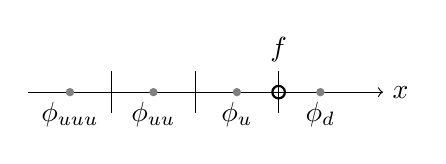
\begin{tikzpicture}[
	  scale=0.53,
	  cpnt/.style={fill=gray},
	]

	\draw [->] (-3,0) -- (5.5,0) node [right] {$x$};
	\draw (-1,-0.5) -- (-1,0.5);
	\draw (1,-0.5) -- (1,0.5);
	\draw (3,-0.5) -- (3,0.5) node [above] {$f$};

	\path [cpnt] (-2,0) circle [radius=0.1] node [below] {$\phi_{uuu}$};
	\path [cpnt] (0,0) circle [radius=0.1] node [below] {$\phi_{uu}$};
	\path [cpnt] (2,0) circle [radius=0.1] node [below] {$\phi_u$};
	\path [cpnt] (4,0) circle [radius=0.1] node [below] {$\phi_d$};
	\draw [thick] (3,0) circle [radius=0.15];
	\end{tikzpicture}
%
	\caption{One-dimensional four-point upwind-biased stencil used to approximate the flux at face $f$.}
	\label{fig:stencil}
\end{figure}

Here we make a comparison between two transport schemes: cubicFit \citep{shaw2017} and highOrderFit, which is based on the high-order formulation by \citet{devendran2017}.  Both schemes form a matrix equation that is solved to find coefficients used to calculate the flux.  We define a one-dimensional, four-point, upwind-biased stencil (figure~\ref{fig:stencil}) with equispaced cell centres.
For cubicFit we approximate a field $\phi$ using a cubic polynomial 
\begin{align}
\phi = a_1 + a_2 x + a_3 x^2 + a_4 x^3
\end{align}
that interpolates the four stencil points.  A matrix equation is formed in order to calculate the unknown coefficients $a_1 \ldots a_4$,
\begin{align}
	\begin{bmatrix}
		1 & x_{uuu} & x_{uuu}^2 & x_{uuu}^3 \\
		1 & x_{uu}  & x_{uu}^2  & x_{uu}^3 \\
		1 & x_u     & x_u^2     & x_u^3 \\
		1 & x_d     & x_d^2     & x_d^3
	\end{bmatrix}
	\begin{bmatrix}
		a_1 \\
		a_2 \\
		a_3 \\
		a_4
	\end{bmatrix}
	=
	\begin{bmatrix}
		\phi_{uuu} \\
		\phi_{uu} \\
		\phi_u \\
		\phi_d
	\end{bmatrix}
	\text{.}
\end{align}
If the equispaced cell centres are positioned at $x_{uuu} = -2.5$, $x_{uu} = -1.5$, $x_u = -0.5$, $x_d = 0.5$ then
\begin{align}
	\begin{bmatrix}
		1 & -2.5 & 6.25 & -15.625 \\
		1 & -1.5 & 2.25 & -3.375 \\
		1 & -0.5 & 0.25 & -0.125 \\
		1 &  0.5 & 0.25 &  0.125
	\end{bmatrix}
	\begin{bmatrix}
		a_1 \\
		a_2 \\
		a_3 \\
		a_4
	\end{bmatrix}
	=
	\begin{bmatrix}
		\phi_{uuu} \\
		\phi_{uu} \\
		\phi_u \\
		\phi_d
	\end{bmatrix}
	\text{.}
	\label{eq:cubicFitMatrix}
\end{align}
For highOrderFit, we solve the matrix equation
\begin{align}
	\begin{bmatrix}
		\moment_{uuu}^0/\moment_{uuu}^0 & \moment_{uuu}^1/\moment_{uuu}^0 & \moment_{uuu}^2/\moment_{uuu}^0 & \moment_{uuu}^3/\moment_{uuu}^0 \\
		\moment_{uu}^0/\moment_{uu}^0 & \moment_{uu}^1/\moment_{uu}^0 & \moment_{uu}^2/\moment_{uu}^0 & \moment_{uu}^3/\moment_{uu}^0 \\
		\moment_u^0/\moment_u^0 & \moment_u^1/\moment_u^0 & \moment_u^2/\moment_u^0 & \moment_u^3/\moment_u^0 \\
		\moment_d^0/\moment_d^0 & \moment_d^1/\moment_d^0 & \moment_d^2/\moment_d^0 & \moment_d^3/\moment_d^0
	\end{bmatrix}
	\begin{bmatrix}
		a_1 \\
		a_2 \\
		a_3 \\
		a_4
	\end{bmatrix}
	=
	\begin{bmatrix}
		\phi_{uuu} \\
		\phi_{uu} \\
		\phi_u \\
		\phi_d
	\end{bmatrix}
\end{align}
where $\moment_V^p = \int_V x^p dV$ is the $p$th moment of volume $V$, and the zeroth moment $\moment_V^0$ is equal to the volume.
If the equispaced cells each have $\moment^0 = 1$ with the cell centres positioned as before, then
\begin{align}
	\begin{bmatrix}
		1 & -2.5 & 6.\dot{3} & -16.25 \\
		1 & -1.5 & 2.\dot{3} & -3.75 \\
		1 & -0.5 & 0.\dot{3} & -0.25 \\
		1 &  0.5 & 0.\dot{3} & 0.25
	\end{bmatrix}
	\begin{bmatrix}
		a_1 \\
		a_2 \\
		a_3 \\
		a_4
	\end{bmatrix}
	=
	\begin{bmatrix}
		\phi_{uuu} \\
		\phi_{uu} \\
		\phi_u \\
		\phi_d
	\end{bmatrix}
	\text{.}
	\label{eq:highOrderMatrix}
\end{align}
Notice how the matrix in equation~\eqref{eq:highOrderMatrix} is similar to, but not equal to, the matrix in equation~\eqref{eq:cubicFitMatrix}.

\section*{Taylor series analysis}

\begin{figure}
	\centering
	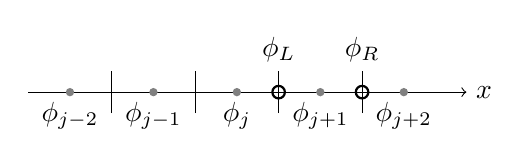
\begin{tikzpicture}[
	  scale=0.53,
	  cpnt/.style={fill=gray},
	]
	\draw [->] (-5,0) -- (5.5,0) node [right] {$x$};
	\draw (-3,-0.5) -- (-3,0.5);
	\draw (-1,-0.5) -- (-1,0.5);
	\draw (1,-0.5) -- (1,0.5) node [above] {$\phi_L$};
	\draw (3,-0.5) -- (3,0.5) node [above] {$\phi_R$};

	\path [cpnt] (-4,0) circle [radius=0.1] node [below] {$\phi_{j-2}$};
	\path [cpnt] (-2,0) circle [radius=0.1] node [below] {$\phi_{j-1}$};
	\path [cpnt] (0,0) circle [radius=0.1] node [below] {$\phi_j$};
	\path [cpnt] (2,0) circle [radius=0.1] node [below] {$\phi_{j+1}$};
	\path [cpnt] (4,0) circle [radius=0.1] node [below] {$\phi_{j+2}$};
	\draw [thick] (1,0) circle [radius=0.15];
	\draw [thick] (3,0) circle [radius=0.15];
	\end{tikzpicture}
	\caption{One-dimensional fluxes through a cell $\phi_{j+1}$ using four-point upwind-biased stencils to approximate fluxes $\phi_L$ and $\phi_R$.}
	\label{fig:flux}
\end{figure}

To find a polynomial that interpolates the 4-point upwind-biased stencil we construct Taylor series approximations centred at $\phi_L$ for the stencil points $\phi_{j-2} \ldots \phi_{j+1}$
\begin{align}
	\begin{bmatrix}
		1 & -\frac{5}{2} & \frac{1}{2!} \left(-\frac{5}{2}\right)^2 & \frac{1}{3!} \left(-\frac{5}{2}\right)^3 \\[4pt]
		1 & -\frac{3}{2} & \frac{1}{2!} \left(-\frac{3}{2}\right)^2 & \frac{1}{3!} \left(-\frac{3}{2}\right)^3 \\[4pt]
		1 & -\frac{1}{2} & \frac{1}{2!} \left(-\frac{1}{2}\right)^2 & \frac{1}{3!} \left(-\frac{1}{2}\right)^3 \\[4pt]
		1 & \frac{1}{2} & \frac{1}{2!} \left(\frac{1}{2}\right)^2 & \frac{1}{3!} \left(\frac{1}{2}\right)^3
	\end{bmatrix}
	\begin{bmatrix}
		\phi_L \\
		\phi'_L \\
		\phi''_L \\
		\phi'''_L
	\end{bmatrix}
	&=
	\begin{bmatrix}
		\phi_{j-2} \\
		\phi_{j-1} \\
		\phi_j \\
		\phi_{j+1}
	\end{bmatrix}
	\text{.}
\end{align}
Solving this system results in the fourth-order accurate approximation, 
\begin{align}
	\phi_L = \frac{1}{16} \phi_{j-2} - \frac{5}{16} \phi_{j-1} + \frac{15}{16} \phi_j + \frac{5}{16} \phi_{j+1} + \mathcal{O}(\Delta x^5)
\end{align}
The approximate flux divergence (figure~\ref{fig:flux}) is then 
\begin{align}
	\phi_R - \phi_L = -\frac{1}{16} \phi_{j-2} + \frac{6}{16} \phi_{j-1} - \frac{20}{16} \phi_j + \frac{20}{16} \phi_{j+1} + \frac{5}{16} \phi_{j+2} \label{eq:cubicFitCoeffs}
\end{align}
but this not a fourth-order accurate flux divergence approximation as we will see next.
A fourth-order accurate approximation to the flux divergence is derived from a Taylor series approximation of $\partial \phi / \partial x$ centred at $\phi_{j+1}$ (figure~\ref{fig:flux}),

\begin{align}
	\begin{bmatrix}
		1 & -3 & \frac{1}{2!} \left(-3\right)^2 & \frac{1}{3!} \left(-3\right)^3 & \frac{1}{4!} \left(-3\right)^4 \\[4pt]
		1 & -2 & \frac{1}{2!} \left(-2\right)^2 & \frac{1}{3!} \left(-2\right)^3 & \frac{1}{4!} \left(-2\right)^4 \\[4pt]
		1 & -1 & \frac{1}{2!} \left(-1\right)^2 & \frac{1}{3!} \left(-1\right)^3 & \frac{1}{4!} \left(-1\right)^4 \\[4pt]
		1 & 0 & \frac{1}{2!} 0^2 & \frac{1}{3!} 0^3 & \frac{1}{4!} 0^4 \\[4pt]
		1 & 1 & \frac{1}{2!} 1^2 & \frac{1}{3!} 1^3 & \frac{1}{4!} 1^4
	\end{bmatrix}
	\begin{bmatrix}
		\phi_{j+1} \\[4pt]
		\phi'_{j+1} \\[4pt]
		\phi''_{j+1} \\[4pt]
		\phi'''_{j+1} \\[4pt]
		\phi''''_{j+1}
	\end{bmatrix}
	&=
	\begin{bmatrix}
		\phi_{j-2} \\
		\phi_{j-1} \\
		\phi_j \\
		\phi_{j+1} \\
		\phi_{j+2}
	\end{bmatrix} \label{eq:highOrderFluxDiv}
\intertext{which yields}
\left. \frac{\partial \phi}{\partial x} \right|_{j+1} = -\frac{1}{12} \phi_{j-2} + \frac{6}{12} \phi_{j-1} - \frac{18}{12} \phi_j + \frac{10}{12} \phi_{j+1} + \frac{3}{12} \phi_{j+2} + \mathcal{O}(\Delta x^4) \text{.} \label{eq:highOrderFluxDivCoeffs}
\end{align}
To find the fourth-order face flux we invert the matrix in equation~\eqref{eq:highOrderMatrix} and find that
\begin{align}
	\phi_L = \frac{1}{12} \phi_{j-2} - \frac{5}{12} \phi_{j-1} + \frac{13}{12} \phi_j + \frac{3}{12} \phi_{j+1} \text{.} \label{eq:highOrderFlux}
\end{align}
Using equation~\eqref{eq:highOrderFluxDiv} and equation~\eqref{eq:highOrderFlux} we can verify that $\left. \partial \phi / \partial x \right|_{j+1} = \phi_R - \phi_L + \mathcal{O}(\Delta x^4)$ as desired (figure~\ref{fig:fluxDivComparison}).

\begin{figure}
	\centering
	\includegraphics[width=5in]{interim-results/taylor-series.png}
	\caption{Flux divergence cofficients using a 5-point Taylor series approximation (equation~\ref{eq:highOrderFluxDivCoeffs}), cubicFit approximation (equation~\ref{eq:cubicFitCoeffs}) and highOrderFit approximation (equation~\ref{eq:highOrderFlux}).}
	\label{fig:fluxDivComparison}
\end{figure}

\bibliographystyle{ametsoc2014}
\bibliography{matrix-comparison}

\end{document}
